\section{User Interface}
This section will look at how each of the designed UI aspects were implemented. UI implementation made use of controllers, which were responsible for conducting database interactions and returning the relevant view, along with HTML, CSS and Javascript for page structure, design and usability. Implementation for different UI components was identical to the concept designs discussed in Chapter \ref{Chapter:Design}.

\subsection{Navigation}
Figure \ref{fig:NavImplementation} shows the implemented navigation bars for unauthorised and unauthorised users. Users are able to navigate to the pages represented by each of the icons on the navigation bar. 

\begin{figure}[H]
	\centering
	\begin{subfigure}{1\linewidth}
		
\includegraphics[width=1\textwidth]{Images/Design/nav-unauthorised}
		\caption{Guest}
		\label{fig:NavUnauth}
	\end{subfigure}
	\begin{subfigure}{1\linewidth}
		
\includegraphics[width=1\textwidth]{Images/Design/nav-authorised}
		\caption{Authorised User}
		\label{fig:NavAuth}
	\end{subfigure}
	\caption{Fidelis navigation bar for (a) unauthorised and (b) authorised users}
	\label{fig:NavImplementation}
\end{figure}

\subsubsection{Links}
Routes for each of the icons are populated using the \textit{LayoutComposer} class, which is a class method that is called whenever the Layout view is rendered \cite{Laravel:Views}. The navigation bar is rendered in the Layout view. Depending on whether the user is authorised or not, the composer returns the title, icon name, route and CSS properties of the relevant icon. Figure \ref{fig:LayoutComposerNav} shows the navigation options for user and application navigation.

\begin{figure}[H]
\centering
\begin{subfigure}[b]{1\linewidth}
	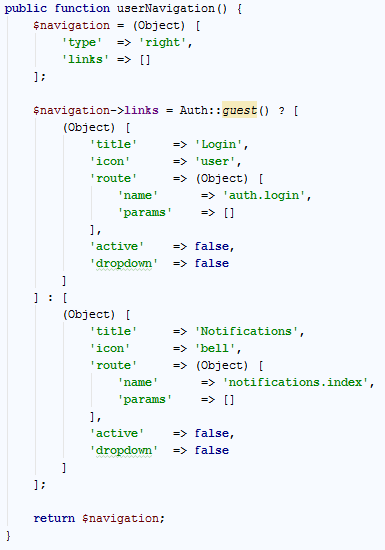
\includegraphics[width=1\textwidth]{Images/Implementation/UserNavigation}
	\caption{}
	\label{fig:UserNavigation}
\end{subfigure}
\begin{subfigure}[b]{1\linewidth}
	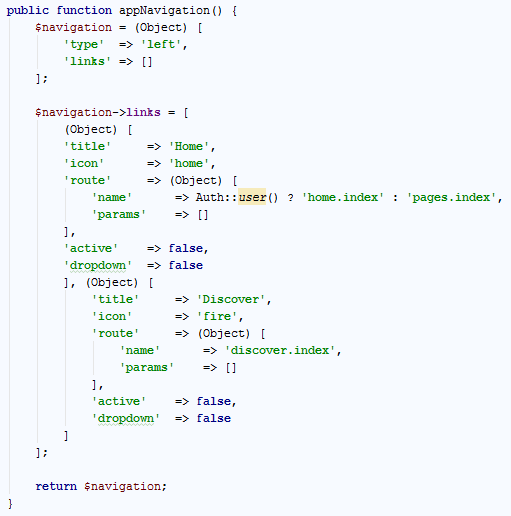
\includegraphics[width=1\textwidth]{Images/Implementation/AppNavigation}
	\caption{}
	\label{fig:AppNavigation}
\end{subfigure}
\caption{Rendering options for (a) user and (b) application navigation}
\label{fig:LayoutComposerNav}
\end{figure}

\subsubsection{Search}
The search bar allows users to enter a query term, and any user or tag matching this search term is retrieved. Using jQuery and JSON, it is possible to live-update the results from the supplied query term and display them to the user. Doing this removes the need to re-direct the user to a separate page which displays the search results to them. An API call to the \textit{SearchController} is made, in which all users and tags matching the query term are retrieved and returned to the view as a JSON object. Figure \ref{fig:SearchController} shows the retrieval of results that match the search term.

\begin{figure}[H]
\centering
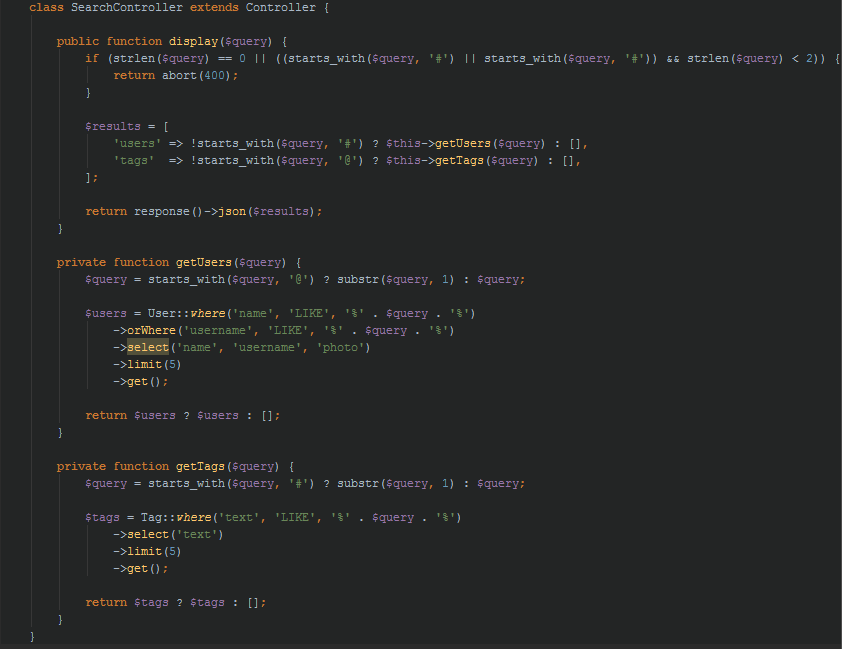
\includegraphics[width=1\textwidth]{Images/Implementation/SearchController}
\caption{Processing of query term performed in \textit{SearchController}}
\label{fig:SearchController}
\end{figure}

It is also possible to search specifically for a user or tag by preceding the query term with a \textbf{@} or \textbf{\#} respectively. Doing this restricts the results returns from the search to just users or tags. In Figure \ref{fig:SearchResults} we can see the implemented search bar, showing the results of providing ``H'' as a query term.

\begin{figure}[H]
\centering
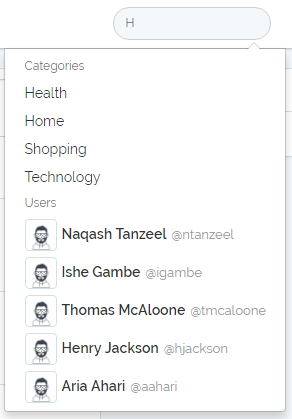
\includegraphics[height=2in]{Images/Implementation/SearchResults}
\caption{Results from searching for the term ``H''}
\label{fig:SearchResults}
\end{figure}

\subsection{Authentication}
Laravel provides built-in functionality for handling user authentication. With this, a number of controllers are available that manage authentication for user login, registration and password recovery \cite{Laravel:Authentication}. By executing the \textit{php artisan make:auth} command, all views and controllers related to user authentication are generated. This command also generates the routes required to navigate to the views, and access controller functionality.

\subsubsection{Registration}
The registration page, shown in Figure \ref{fig:RegisterPage}, collects the users' name, email address, username, date of birth, password, and also asks the user to agree with the Fidelis terms of service. If the user provides all the required fields, they are re-directed to the home page. The post-authentication redirection location can be modified in the \textit{RegisterController}.

\begin{figure}[H]
\centering
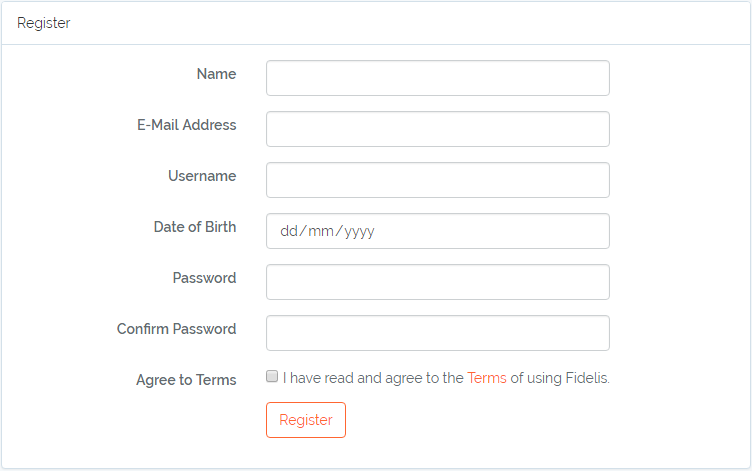
\includegraphics[height=2in]{Images/Design/register-page}
\caption{Registration page}
\label{fig:RegisterPage}
\end{figure}

In addition to the redirection location, the \textit{RegisterController} contains \texttt{validator()} and \texttt{create()} functions. Before the user is redirected to the home page on successful authentication, the controller first applies a set of validation rules specified in the validator (Figure \ref{fig:RegValidation}) which must be verified before the user is authenticated. If validation is correct, the new user is created with the \texttt{create()} function and authenticated (Figure \ref{fig:register-controller}), leading to successful redirection.

\begin{figure}[H]
\centering
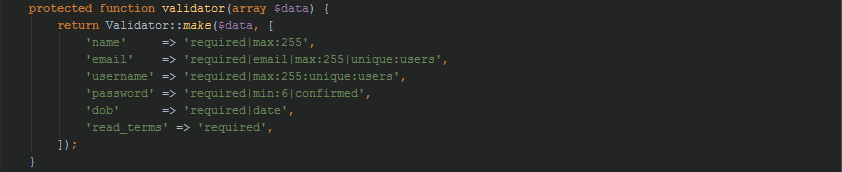
\includegraphics[width=\textwidth]{Images/Implementation/RegisterValidation}
\caption{Validation rules applies to fields supplied by user on the Registration page}
\label{fig:RegValidation}
\end{figure}

\subsubsection{Login}
The login page, shown in Figure \ref{fig:LoginPage}, requests the users' email address and password. Similarly to registration, users who are successfully authenticated are redirected to the home page. All authentication functionality is handled by the pre-built \textit{LoginController}. If incorrect account credentials are provided, authentication is unsuccessful.

\begin{figure}[H]
\centering
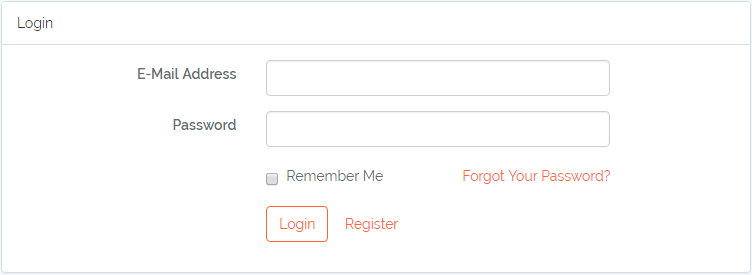
\includegraphics[height=1.5in]{Images/Design/login-page}
\caption{Log-in page}
\label{fig:LoginPage}
\end{figure}

\subsubsection{Password Reset}
The password reset page, shown in Figure \ref{fig:PasswordReset} allows users to reset their passwords if they have forgotten their account credentials. By navigating to this page, users can submit a form containing their email addressing. Submission of this form will prompt the \textit{ResetController}, which handles password resetting using pre-built functionality, to send a password reset link to the provided email address if an account exists for that address.

\begin{figure}[H]
\centering
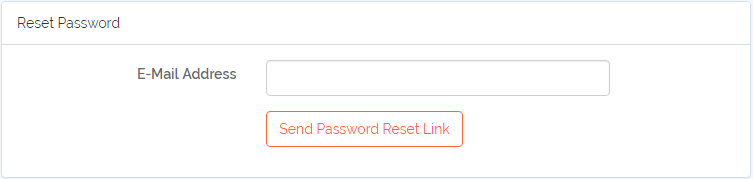
\includegraphics[height=1in]{Images/Implementation/PasswordReset}
\caption{Account recovery page}
\label{fig:PasswordReset}
\end{figure}

\subsection{Home}
When a user first navigates to the Fidelis platform - either for the first time, or if they are not logged into an account - they will be faced with the landing page shown in Figure \ref{fig:HomeUnauthorised}.  

\begin{figure}[H]
\centering
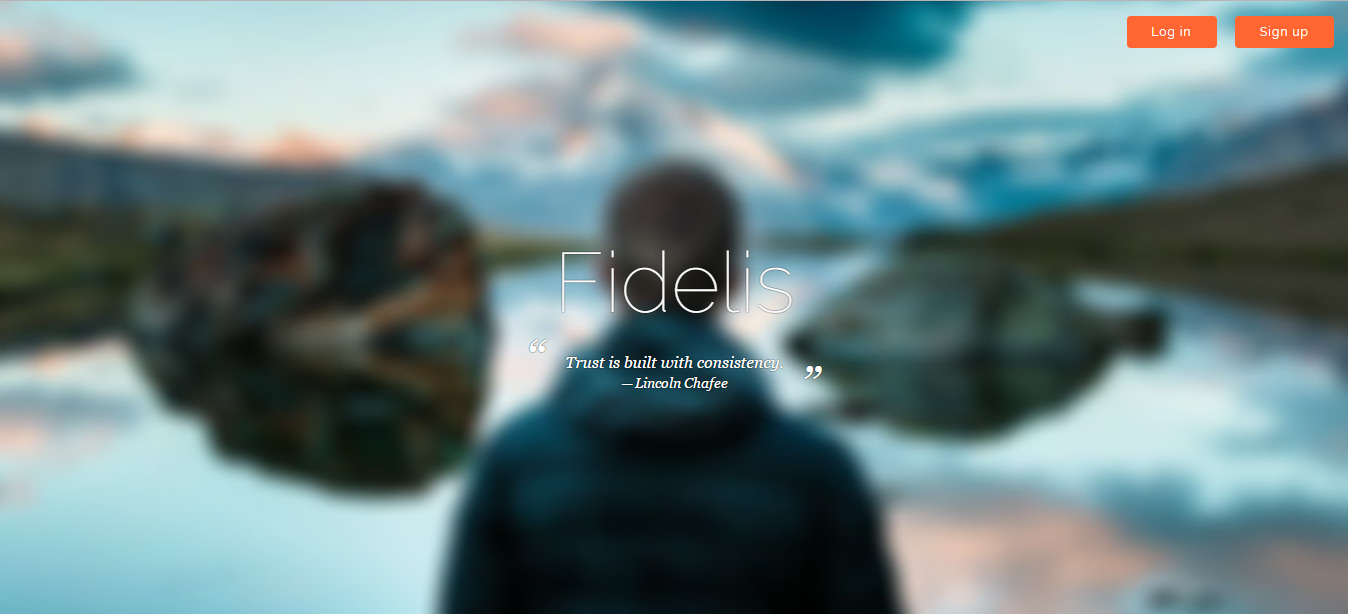
\includegraphics[width=\textwidth]{Images/Implementation/home_unauthorised}
\caption{Landing Page}
\label{fig:HomeUnauthorised}
\end{figure}

This landing page is created by the view shown in Figure \ref{fig:LandingView}. We can see that if the user is detected to be a guessed, i.e., not logged into an account, this page will be shown. The view provides two buttons at the top right of the page, one for logging into an existing account, and one for signing up for a new account. In addition, a background wallpaper will be provided randomly from a number of stored image assets. Finally the title of the website, `Fidelis', is displayed along with a quote (and a name of the person to whom the quote is attributed) regarding trust: the central theme of Fidelis.

\begin{figure}[H]
\centering
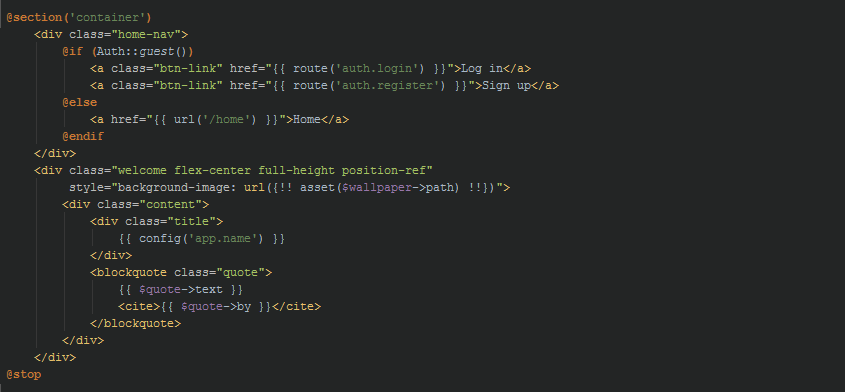
\includegraphics[width=\textwidth]{Images/Implementation/LandingView}
\caption{Landing page view}
\label{fig:LandingView}
\end{figure}

If, however it is determined that the user is logged in when they navigate to this page, they will be routed from this landing page to the home page shown in Figure \ref{fig:HomeAuthorised}.

\begin{figure}[H]
\centering
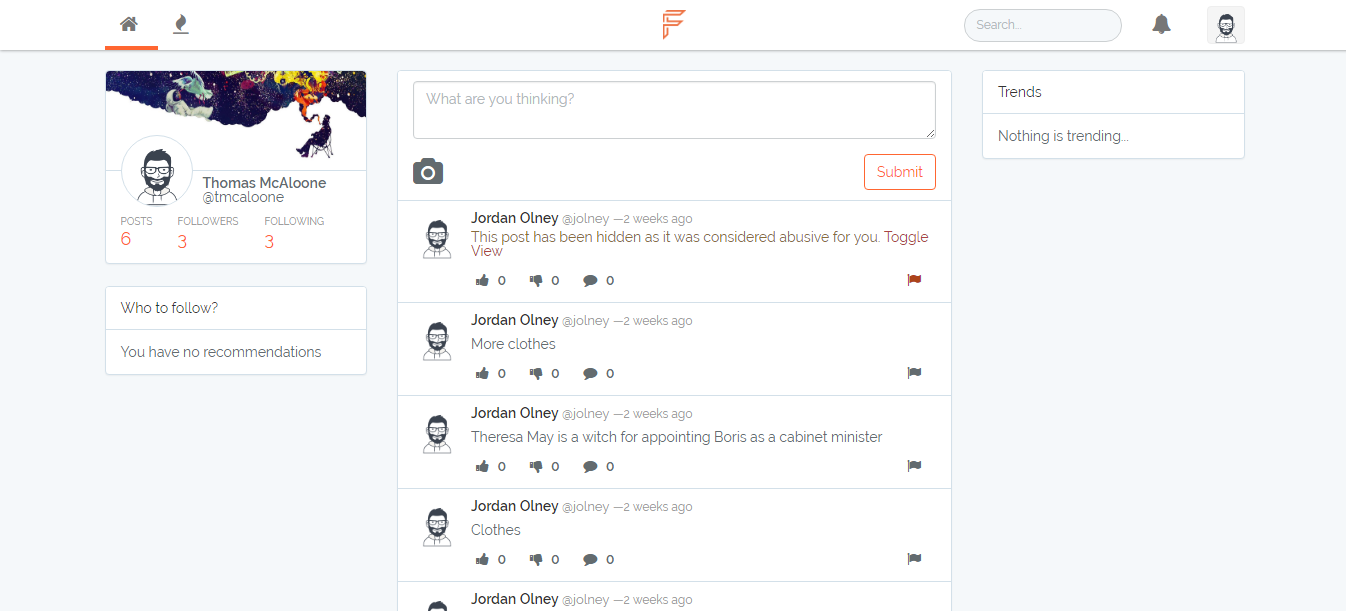
\includegraphics[width=\textwidth]{Images/Implementation/home_authorised}
\caption{Home Page}
\label{fig:HomeAuthorised}
\end{figure}

Upon the user being directed to the home page, a call will be made to the $index()$ function of the $HomeController$ via the routing. Figure \ref{fig:HomeRoutingController} shows this route as well as the $index$ function. The $index()$ function will first find the user id of each other account that the user is following. Then it will find all posts belonging to all of these users. The posts found are then returned to the home page to be displayed in order from the most recent post to the oldest post.

\begin{figure}[H]
\centering
\begin{subfigure}[b]{1\linewidth}
	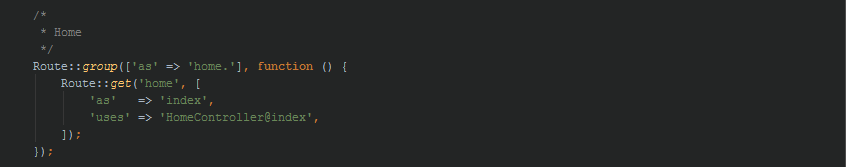
\includegraphics[width=\textwidth]{Images/Implementation/HomeRouting}
	\caption{}
	\label{fig:HomeRouting}
\end{subfigure}
\begin{subfigure}[b]{1\linewidth}
	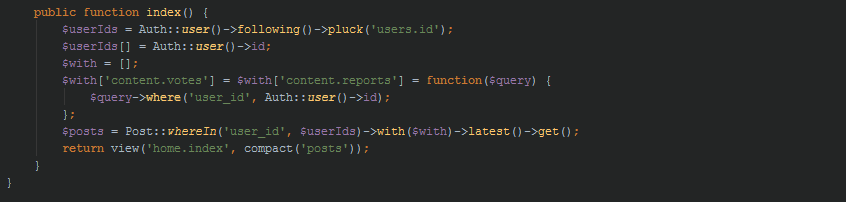
\includegraphics[width=1\textwidth]{Images/Implementation/HomeControllerIndexFunction}
	\caption{}
	\label{fig:HomeControllerIndexFunction}
\end{subfigure}
\caption{(a) Home page routing and (b) $index()$ function of the $HomeController$}
\label{fig:HomeRoutingController}
\end{figure}

Once the posts from accounts the user is following have loaded in, the user also has the ability to create and share their own content. The user can type their own text to post as well as being able to upload an image with the post. Figure \ref{fig:HomeNewPostForm} shows the AJAX form involved with creating a new post. The user can type text into the available text area to be submitted with the post.

\begin{figure}[H]
\centering
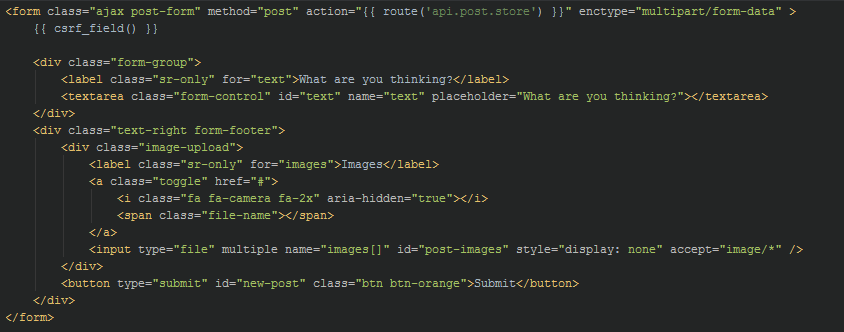
\includegraphics[width=\textwidth]{Images/Implementation/HomeNewPostForm}
\caption{AJAX form for creating a new post}
\label{fig:HomeNewPostForm}
\end{figure}

In addition, there is an icon which can be clicked to upload a photo with the post. Figure \ref{fig:HomeNewPostAJAX} shows the AJAX code that is used to handle image uploads and form submission. Firstly, this code finds the class involved with uploading a photo and waits for the upload icon to be clicked. Once this happens, the user will choose an image to upload and upon them doing so, the code will attain the filename of the image and display it next to the icon. If the user chooses to upload more than one image, `$n$ Files' will be displayed instead, where `$n$' is the number of files being uploaded.

The rest of the code handles the submission of the form (Once the user hits submit to create the post). At this point, the new post will be automatically categorised using the script $predict.py$. The URL for this form submission is seen to be the form's `action' attribute. Looking at the first line of \ref{fig:HomeNewPostForm} again we can see that the form is set up to route a post request using the $store()$ function in the $PostController$. This function simply stores the new post in the database and then returns the same post to the home page. This post will then appear at the top of the home page for the user.

\begin{figure}[H]
\ContinuedFloat
\centering
\begin{subfigure}[b]{1\linewidth}
	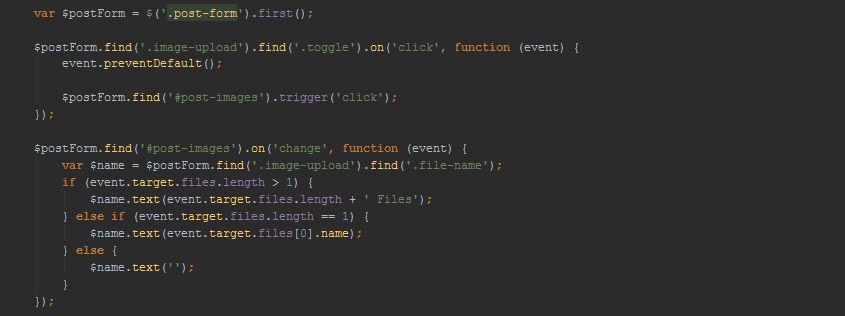
\includegraphics[width=\textwidth]{Images/Implementation/HomeNewPostJS}
	\caption{}
	\label{fig:HomeNewPostJS}
\end{subfigure}
\end{figure}
\begin{figure}[H]\ContinuedFloat
\begin{subfigure}[b]{1\linewidth}
	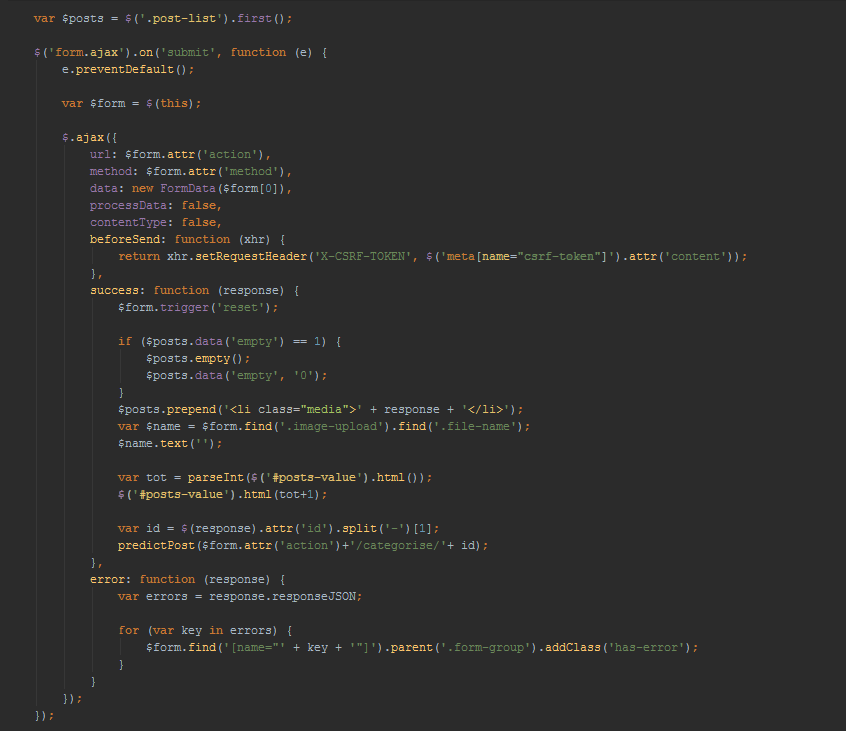
\includegraphics[width=\textwidth]{Images/Implementation/HomeNewPostJS2}
	\caption{}
	\label{fig:HomeNewPostJS2}
\end{subfigure}
\caption{AJAX function for handling a new post: (a) inserting and image and (b) submitting the form}
\label{fig:HomeNewPostAJAX}
\end{figure}

\subsection{Discover}
The implemented discover page is shown in Figure \ref{fig:DiscoverPage}. This page gives the ability for a user to seek out and find new content, which appeals to them, outside of the content they see from their current network. The user can used this page to find new content from specific categories, see content from tags they have subscribed to (and manage these subscriptions), as well as seeing content recommended for them.

\begin{figure}[H]
\centering
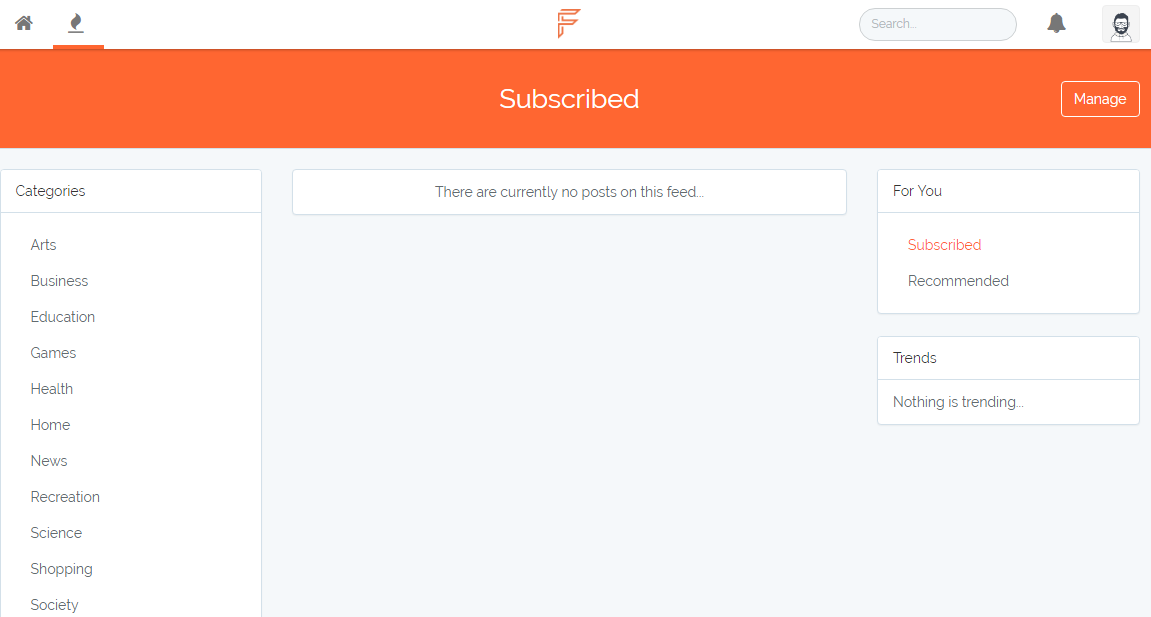
\includegraphics[width=\textwidth]{Images/Implementation/DiscoverPage}
\caption{Discover Page}
\label{fig:DiscoverPage}
\end{figure}

The banner seen across the top of the page contains the title of the current page. The title that is shown therefore depends on which data is being displayed. For each case a separate view has been created to display the correct title. This is usually the name of the category, however there are exceptions for viewing the user's subscriptions - in which case a button must also be included to link to the Settings page where the user can manage their subscriptions - as well as viewing the user's recommended content. Figure \ref{fig:DiscoverTitle} shows these different views.

\begin{figure}[H]
\centering
\begin{subfigure}[b]{1\linewidth}
	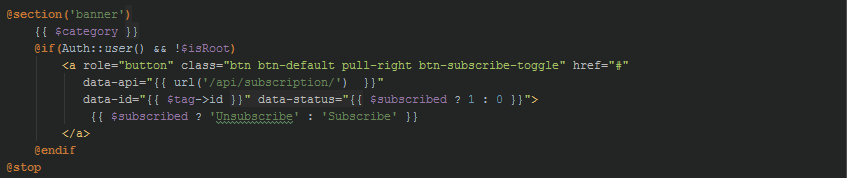
\includegraphics[width=\textwidth]{Images/Implementation/CategoryBladePhp}
	\caption{}
	\label{fig:CategoryBladePhp}
\end{subfigure}
\begin{subfigure}[b]{1\linewidth}
	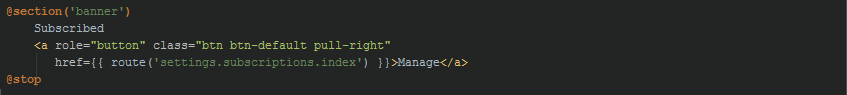
\includegraphics[width=\textwidth]{Images/Implementation/IndexBladePhp}
	\caption{}
	\label{fig:IndexBladePhp}
\end{subfigure}
\begin{subfigure}[b]{1\linewidth}
	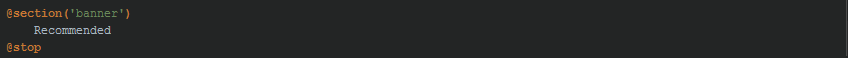
\includegraphics[width=\textwidth]{Images/Implementation/RecommendedBladePhp}
	\caption{}
	\label{fig:RecommendedBladePhp}
\end{subfigure}
\caption{Different view outputs of Title for (a) Categories, (b) Subscribtions and (c) Recommendations}
\label{fig:DiscoverTitle}
\end{figure}

In order to determine which content needs to be loaded to the post feed, the system determines which option is `active', i.e., whether the user has selected to view content they are subscribed to, content recommended for them, or content from a category. For each of these options there is a corresponding route to follow. These routes are shown in Figure \ref{fig:DiscoverRouting}.

\begin{figure}[H]
\centering
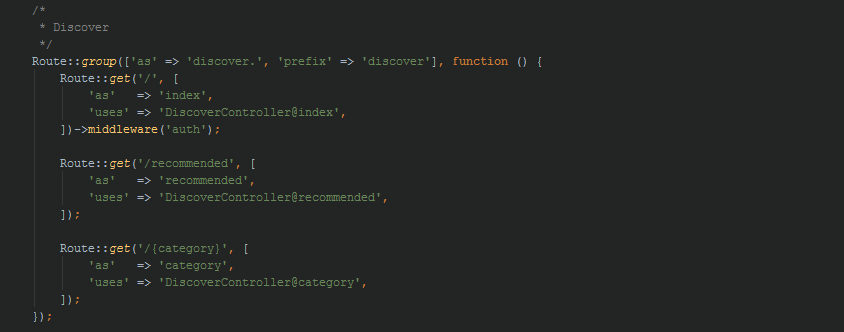
\includegraphics[width=\textwidth]{Images/Implementation/DiscoverRouting}
\caption{Discover Routing}
\label{fig:DiscoverRouting}
\end{figure}

\subsubsection{Discover Controller Actions}
Each of these routes followed from the discover page result in a different action being taken by the $DiscoverController$. Note that routing to the index route (for subscriptions) here requires a check to ensure the user is authorised to take that action (check the user is signed into an account since otherwise they will have no subscriptions). Each of these actions will ultimately return a number of posts (and relevant data regarding those posts) from the database to be handled by the discover page (displaying those posts in the posts feed).

\paragraph{Subscribed Content}
When the discover page needs to display content the user is subscribed to, the $index()$ function of the $DiscoverController$ is called. This function is shown in Figure \ref{fig:DiscoverControllerSubscribed}. This function will retrieve the id of every tag the user is subscribed to. The function then collects every posts which has a tag, where that tag is one that the user is subscribed to. These posts are then returned to the discover page to be displayed in order from the most recent to the oldest post.

\begin{figure}[H]
\centering
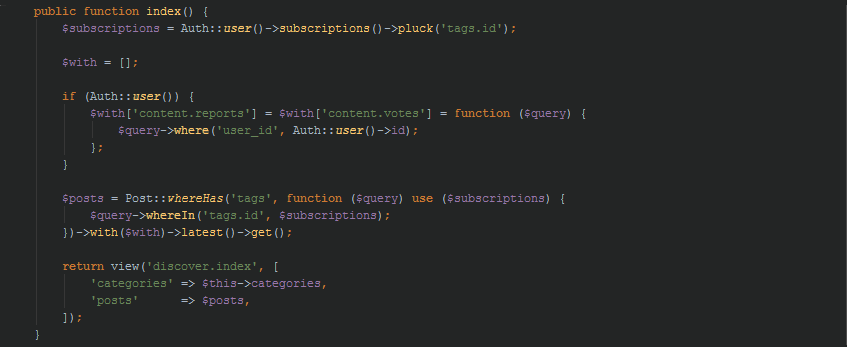
\includegraphics[width=\textwidth]{Images/Implementation/DiscoverControllerSubscribed}
\caption{Discover Controller action for displaying subscribed content}
\label{fig:DiscoverControllerSubscribed}
\end{figure}

\paragraph{Recommended Content}
When the discover page needs to display content that is recommended for the current user, the $recommend()$ function of the $Discover  Controller$ is called. This function is shown in Figure \ref{fig:DiscoverControllerSubscribed}. The function will call the $recommendedPosts()$ function shown in Figure \ref{fig:RecommendedPosts}. The $recommendedPosts()$ function simply returns all posts that are recommended to the given user. These posts are then returned to the discover page to be displayed in order from the most recent to the oldest post.

\begin{figure}[H]
\centering
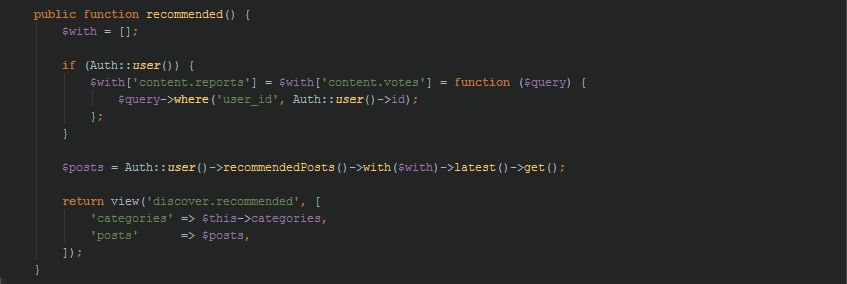
\includegraphics[width=\textwidth]{Images/Implementation/DiscoverControllerRecommended}
\caption{Discover Controller action for displaying recommended content }
\label{fig:DiscoverControllerRecommended}
\end{figure}

\begin{figure}[H]
\centering
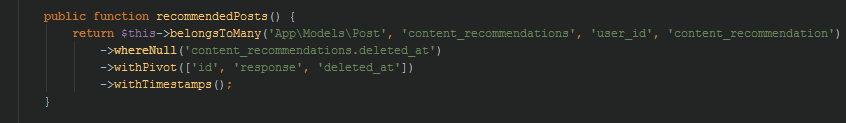
\includegraphics[width=\textwidth]{Images/Implementation/RecommendedPosts}
\caption{$recommendedPosts()$ function}
\label{fig:RecommendedPosts}
\end{figure}

\paragraph{Category Content}
When the discover page needs to display content from a specific category that the user has selected to view, the $category()$ function of the $Discover  Controller$ is called. This function is shown in Figure \ref{fig:DiscoverControllerSubscribed}. After performing a few checks including finding if the $\$category$ variable passed is in fact a category (root tag) or simply a tag belonging to a category. This is because this function is also accessed when the user is routed to the discover page from a trending tag. If it is a root category, the function will find the id of every tag within that category and then find every post with a tag that has a matching tag id. Alternatively, if the variable passed is simply a tag belonging to a category, the function will find all posts using that tag. Either way, these posts are then returned to the discover page to be displayed in order from the most recent to the oldest post.

\begin{figure}[H]
\centering
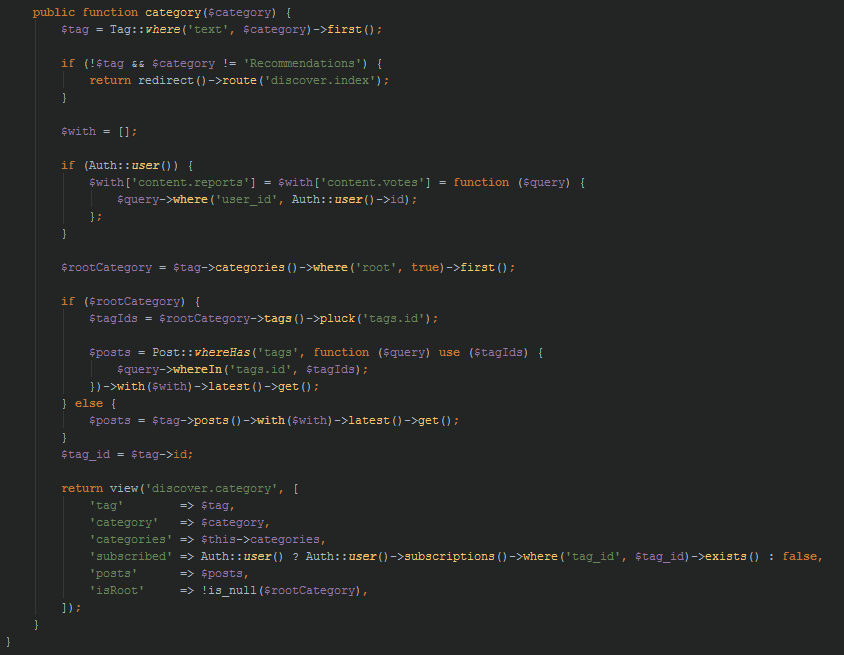
\includegraphics[width=\textwidth]{Images/Implementation/DiscoverControllerCategory}
\caption{Discover Controller action for displaying content from a category}
\label{fig:DiscoverControllerCategory}
\end{figure}

\subsection{Notifications}
Figure \ref{fig:NotificationsPage} shows the implemented notifications page. Users receive a notification whenever they receive a new follow, are mentioned in a post by another user, or one of their posts is commented or voted on. The page provides users with information on the notification type, and if relevant the content of the notification (for example, the comment made on their post). The counter, seen next to the bell icon on the navigation bar, indicates to the user how many unread notifications they have. The notification page only fetches unread notifications, which reduces the amount of data that is retrieved from the database. This speeds up the load time of the page. When the user visits the notifications page, all unread notifications are marked as read. 

\begin{figure}[H]
\centering
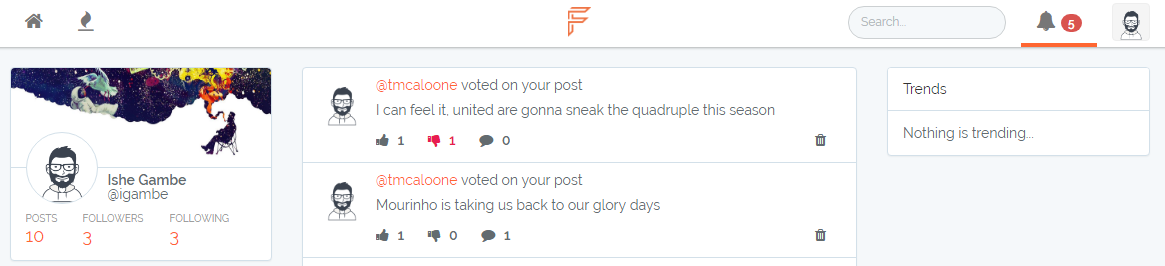
\includegraphics[width=\textwidth]{Images/Implementation/NotificationsPage}
\caption{Notifications Page}
\label{fig:NotificationsPage}
\end{figure}

Laravel provides support for integrating a notification system with your application \cite{Laravel:Notifications}. With this, it is possible to create different notification types, and have these related to a user by using the \texttt{Notification} facade. Using this facade means that whenever an interaction happens with a user or with their posts, they can be notified of this using the \textit{notify()} function:

\begin{lstlisting}[language=bash]
	$user->notify(new NameOfNotification($notification)
\end{lstlisting}

It is also possible to queue notifications. Creating a queue of notifications can speed up application response time as there can be delays when delivering notifications to the user \cite{Laravel:Notifications, Laravel:Queues}. Queueing can be enabled by adding the \textit{Queueable} trait to the notification class, and starting a queue worker by configuring the queue in \textit{config/queue.php}. Figure \ref{fig:CommentNotification} shows the notification class created for comments. The \texttt{toArray()} function contains an array that represents information carried by the notification. In the array we have a `regarding' entry, which represents the item the notification is related to, a `to' entry which represents who the notification is meant for, and a `text' field which contains information displayed to the user receiving the notification.

\begin{figure}[H]
\centering
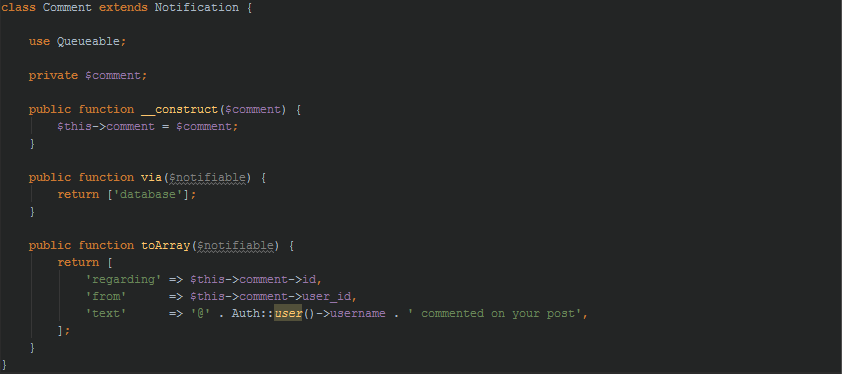
\includegraphics[width=\textwidth]{Images/Implementation/CommentNotification}
\caption{Custom notification for comments}
\label{fig:CommentNotification}
\end{figure}

\subsection{Profile}
The user profile page, shown in Figure \ref{fig:ProfilePage}, allows the user to see all their activity and public information related to their account (Name, bio etc.), as well as reviewing their posts, followers and so on. A user can also view the profiles of other users which creates yet another avenue for discovering new content, as well as nurturing user-to-user interactions across the platform. Upon loading a user's profile page, their cover photo and profile picture will be loaded from the database. On the right of the page we also have the ability to Follow/Unfollow the user, as well as the option to block that user. There is also a widget on the right of the page displaying trending topics.

\begin{figure}[H]
\centering
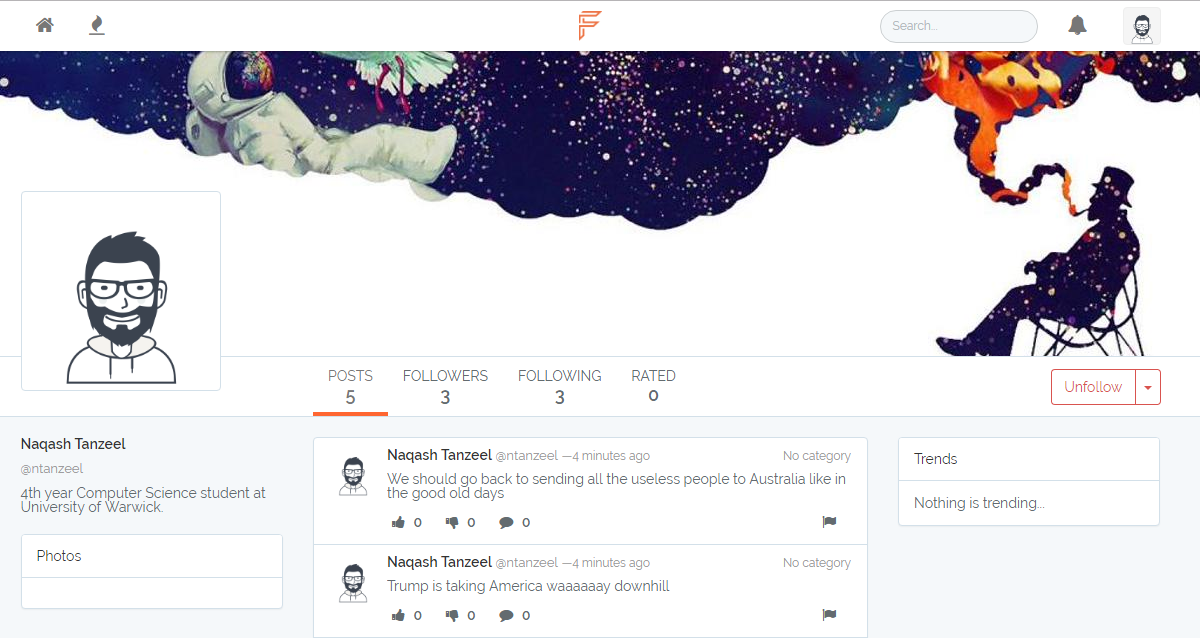
\includegraphics[width=\textwidth]{Images/Implementation/ProfilePage}
\caption{User profile page}
\label{fig:ProfilePage}
\end{figure}

\subsubsection{User activity}
The main feature of this page is the ability to view the activity of this user. This can be done using the 4 tabs in the centre of the page: Posts, Followers, Following and Rated. Each one routes to its own page, each calling upon a different function from the \(ProfileController\). These routes can be seen in Figure \ref{fig:ProfileRouting}.

\begin{figure}[H]
\centering
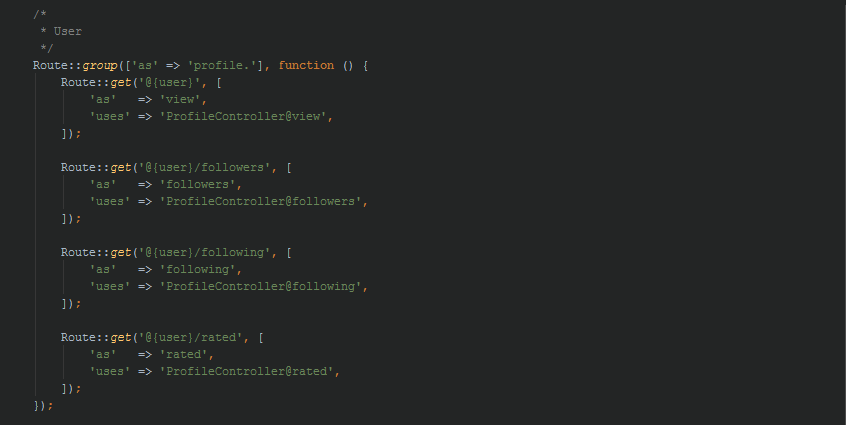
\includegraphics[width=\textwidth]{Images/Implementation/ProfileRouting}
\caption{Routes for the user profile page}
\label{fig:ProfileRouting}
\end{figure}

The posts tab (Figure \ref{fig:ProfilePosts}) calls upon the \(view()\) function from the \(ProfileController\). This function, as with each of the functions called by routes on this page, begins by calling the \(preRoute()\) function, which assesses whether the current user is authorised to view this data (e.g. ensuring the user is logged in, not blocked etc.). Once this is confirmed, the \(view()\) function will find all of the posts from the user who's page is being viewed and return them in order from the most recent post to the oldest post by this user.

\begin{figure}[H]
\centering
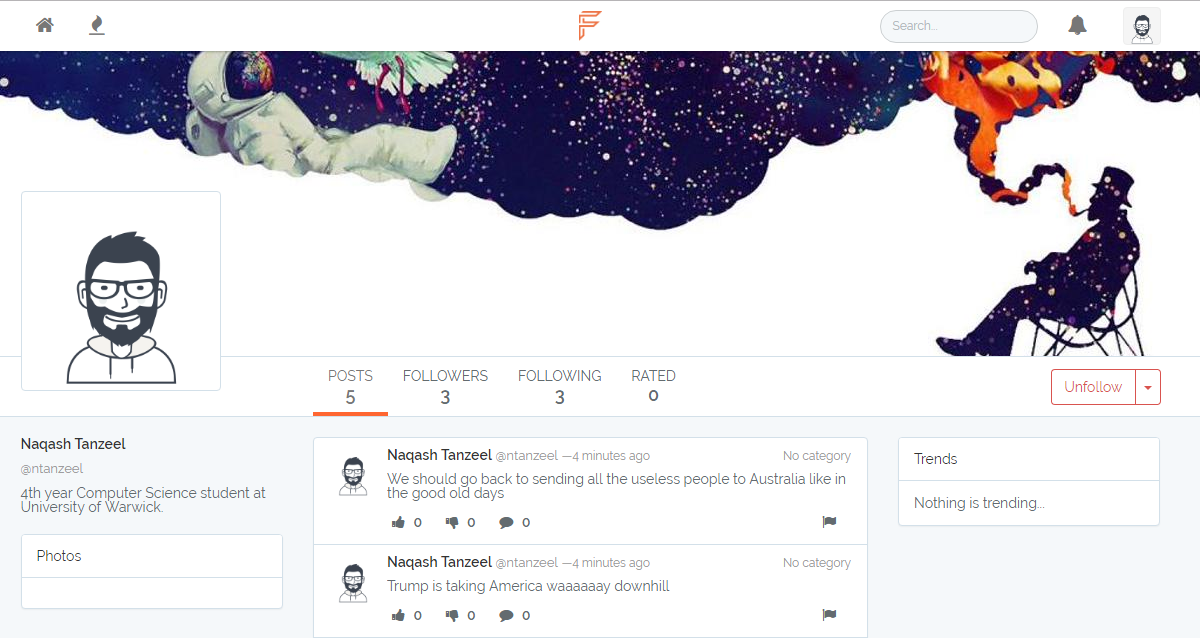
\includegraphics[width=\textwidth]{Images/Implementation/ProfilePosts}
\caption{Posts tab on the user profile page}
\label{fig:ProfilePosts}
\end{figure}

The followers tab (Figure \ref{fig:ProfileFollowers}) calls upon the \(followers()\) function from the \(ProfileController\). This function firstly uses the \(preRoute()\) function, to assess whether the current user is authorised to view this data. Once this is confirmed, the \(followers()\) function will find and return all of the users who follow the user in question. These will then be displayed as a series of user widgets, one for each user following the user to whom the profile belongs. The posts are displayed in a post feed.

\begin{figure}[H]
\centering
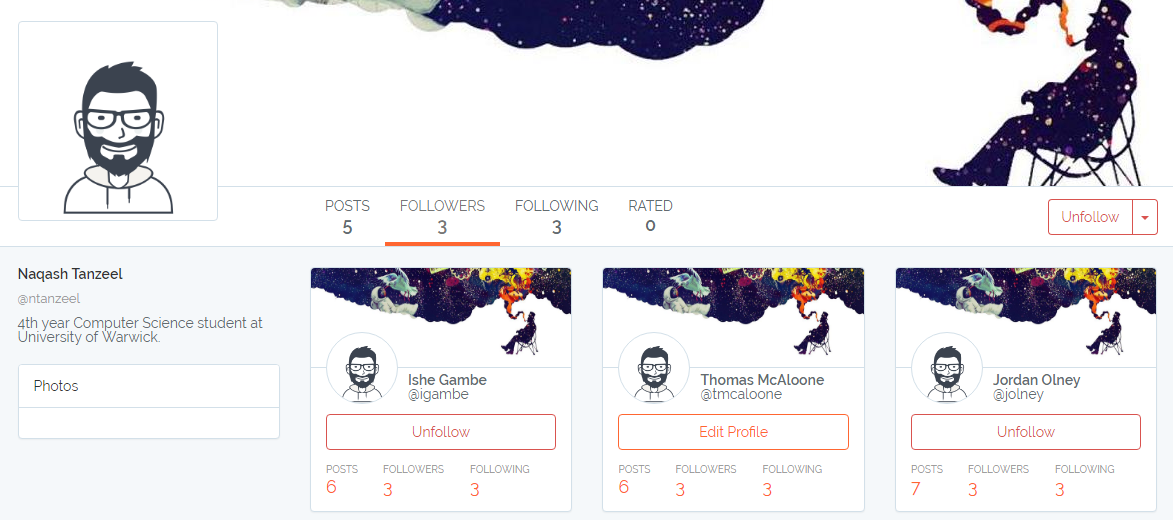
\includegraphics[width=\textwidth]{Images/Implementation/ProfileFollowers}
\caption{Followers tab on the user profile page}
\label{fig:ProfileFollowers}
\end{figure}

In much the same way, the following tab (Figure \ref{fig:ProfileFollowing}) calls upon the \(following()\) function from the \(ProfileController\). This function firstly uses the \(preRoute()\) function, to assess whether the current user is authorised to view this data. Once this is confirmed, the \(following()\) function will find and return all of the users who are followed by the user in question. These will then be displayed as a series of user widgets, one for each user that the user to whom the profile belongs follows.

\begin{figure}[H]
\centering
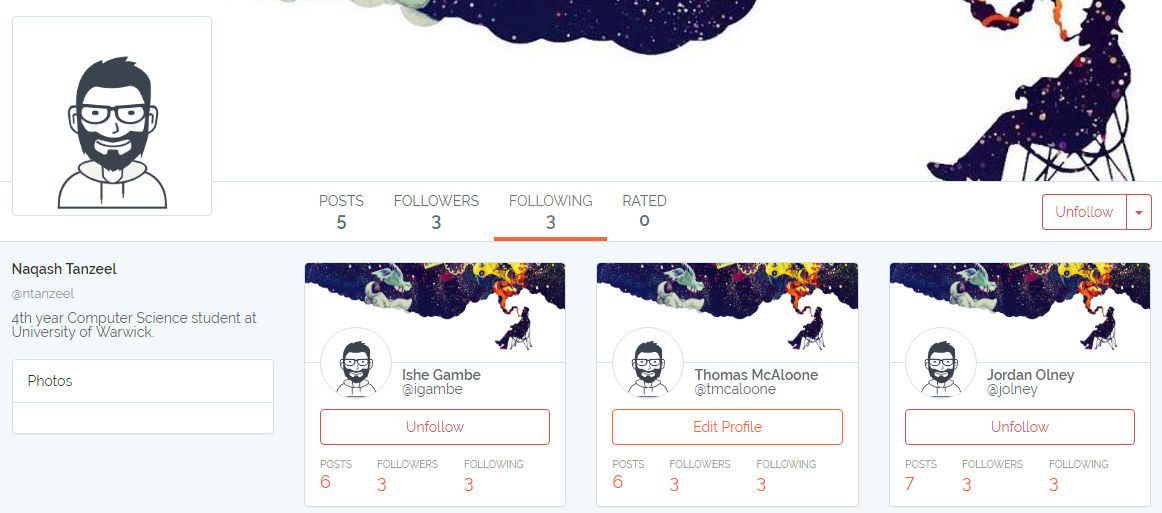
\includegraphics[width=\textwidth]{Images/Implementation/ProfileFollowing}
\caption{Following tab on the user profile page}
\label{fig:ProfileFollowing}
\end{figure}

The rated tab (Figure \ref{fig:ProfileRated}) calls upon the \(rated()\) function from the \(ProfileController\). This function firstly uses the \(preRoute()\) function, to assess whether the current user is authorised to view this data. Once this is confirmed, the \(rated()\) function will find and return all of the posts which the user in question has rated, i.e., has either voted up or voted down. These posts are returned in order from the most recent post to the oldest post by this user. The posts are displayed in a post feed.

\begin{figure}[H]
\centering
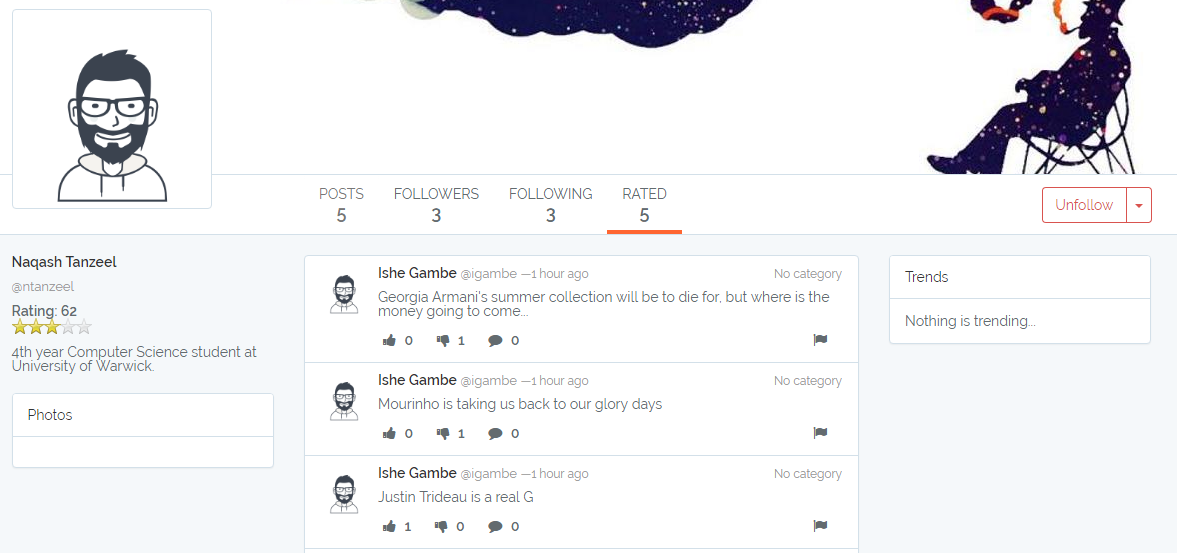
\includegraphics[width=\textwidth]{Images/Implementation/ProfileRated}
\caption{Rated tab on the user profile page}
\label{fig:ProfileRated}
\end{figure}

\subsubsection{Photos Widget}
The photos widget can be seen on the left hand side of a user's profile page. This widget displays photos that a user has uploaded to the Fidelis Platform. Upon the page being loaded, this widget will be populated with the user's photos, retrieved from the database. The images not only appear in the widget, but upon clicking one of the photos, a modal lightbox will popup over the page. The user can use this to look through all of the photos that the user has uploaded.

\subsection{Settings}
Figure \ref{fig:SettingsImplementation} shows the settings page that allows the user to toggle user account settings. The user is able to modify profile and privacy \& safety settings. In addition to this, they can also manage tags they are subscribed to, and user accounts they have blocked.

\begin{figure}[H]
\centering
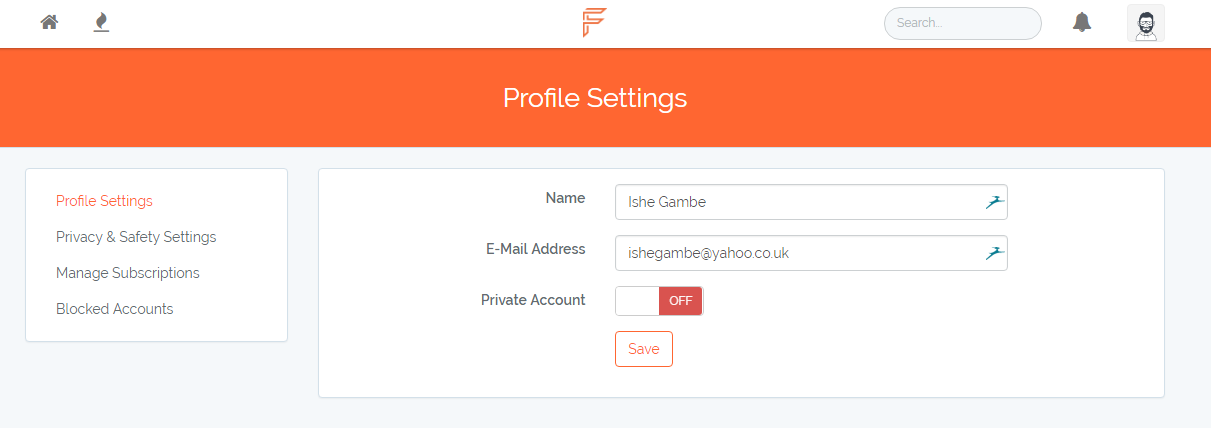
\includegraphics[width=\textwidth]{Images/Implementation/SettingsPage}
\caption{Profile settings from the settings page}
\label{fig:SettingsImplementation}
\end{figure}

Each subset of settings is handled by different controllers. The \textit{AccountController} handles any changes made by the user to their name, email address or the privacy of the account. The controller also handles requests made by the user to edit or upload their profile pictures. The \textit{SafetyController}, seen in Figure \ref{fig:SafetyController}, retrieves the users default settings. As mentioned previously, users are able to modify settings related to abuse detection and recommendations. Before a user has had the chance to modify these settings, default settings are are provided for each user. Default settings are retrieved using the query shown in figure \ref{fig:UserDefaultSettings}. This query is added as a function on the model.

\begin{figure}[H]
\centering
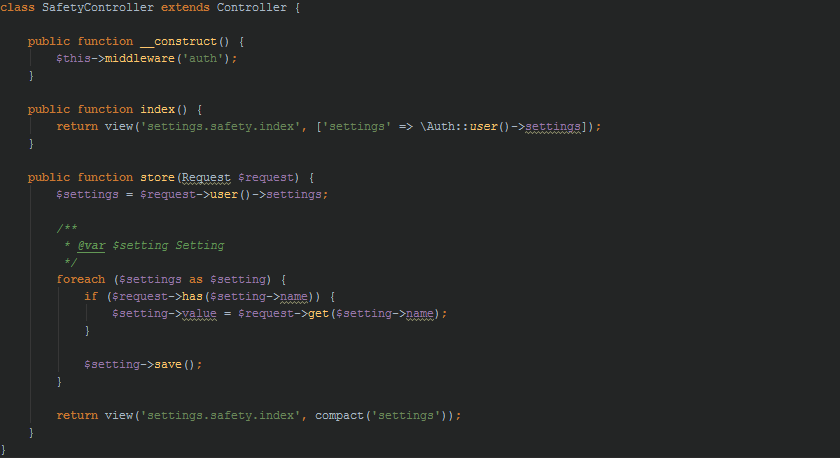
\includegraphics[width=\textwidth]{Images/Implementation/SafetyController}
\caption{Safety Controller}
\label{fig:SafetyController}
\end{figure}

The \textit{SubscriptionsController} returns the users subscriptions in a similar fashion to how default settings are retrieved. The \textit{BlockedController} also follows this approach, using a query to retrieve blocked users defined on the user model to return any blocked users.

\begin{figure}[H]
\centering
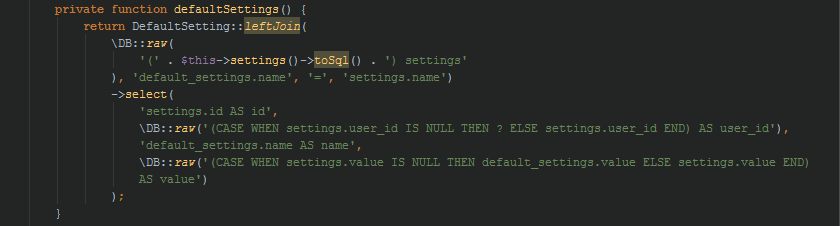
\includegraphics[width=\textwidth]{Images/Implementation/UserDefaultSettings}
\caption{Query to retrieve default settings for the user}
\label{fig:UserDefaultSettings}
\end{figure}

\subsection{Static Pages}
The two static pages aim to address the possible issues discussed in section \ref{Chapter:Issues}, by displaying information about the terms of use for Fidelis and providing support in order to help alleviate any personal issues which can arise through the use of social networking sites. These pages are accessible to both authorised users and guests visiting Fidelis. Both static pages are accessible via links in the footer of every page.

\subsubsection{Support}
The support page displays details of how to deal with content on the site which may distress the user. Fidelis aims to keep this content to a minimum, through the abuse detection, reputation scoring and terms of service, however, some content may still be posted on the platform which is not prevented via these measures. Therefore, the page lists options of how to remove the content, by reporting it and adjusting abuse detection settings. It also provides contact details to the Samaritans \cite{Samaritans:Home}, who can offer support in case of any social issues which may arise on the network such as cyber-bullying. As seen in figure \ref{fig:SupportPage}, the styling for the page is simplistic, using bullet points in order to break down the information being provided.

\begin{figure}[H]
\centering
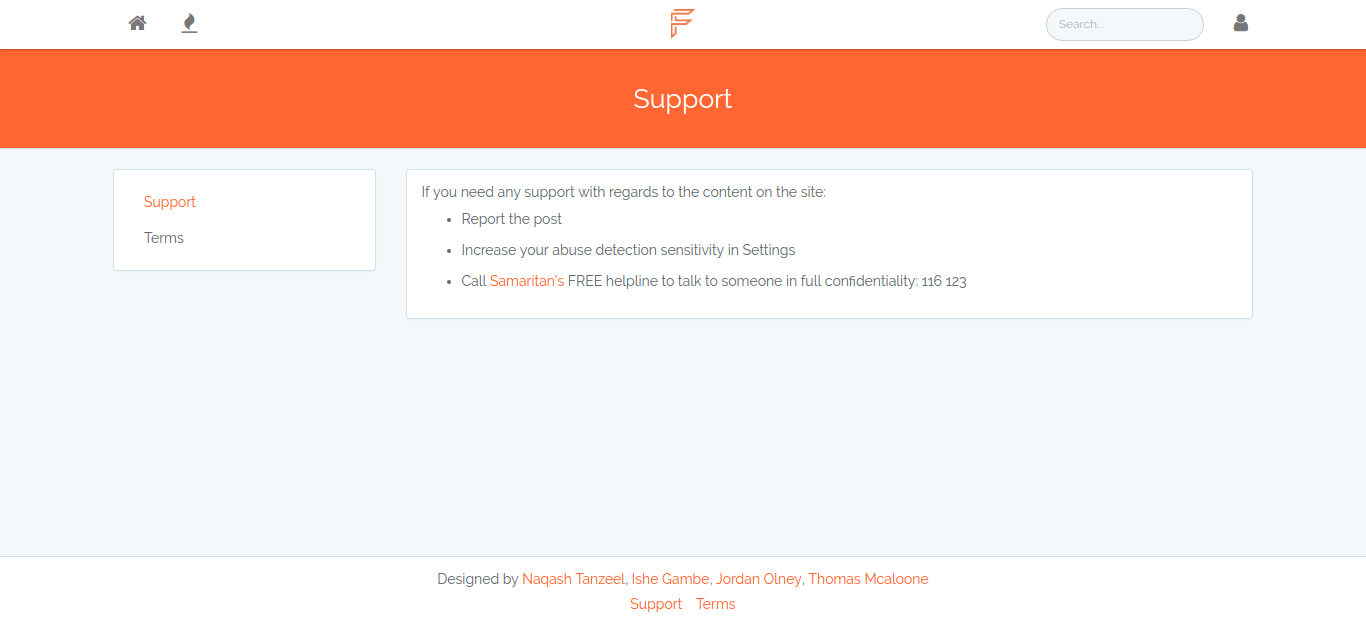
\includegraphics[height=2in]{Images/Design/support-page}
\caption{Design for support page}
\label{fig:SupportPage}
\end{figure}

\subsubsection{Privacy Policy}
The styling for the terms page is the same as the support page, using bullet points to help make the information more readable, as shown in figure \ref{fig:ToS}. The information provided, however, is regarding the terms of service, to ensure that the user understands what is expected of them when using the site and the service Fidelis is expected to provide. This is to help avoid any legal issues which may arise from the content which is posted on the site by users. The Fidelis terms of service were modelled after the Twitter Private Policy \cite{Twitter:PrivatePolicy} and Terms of Service \cite{Twitter:ToS}.

\begin{figure}[H]
\centering
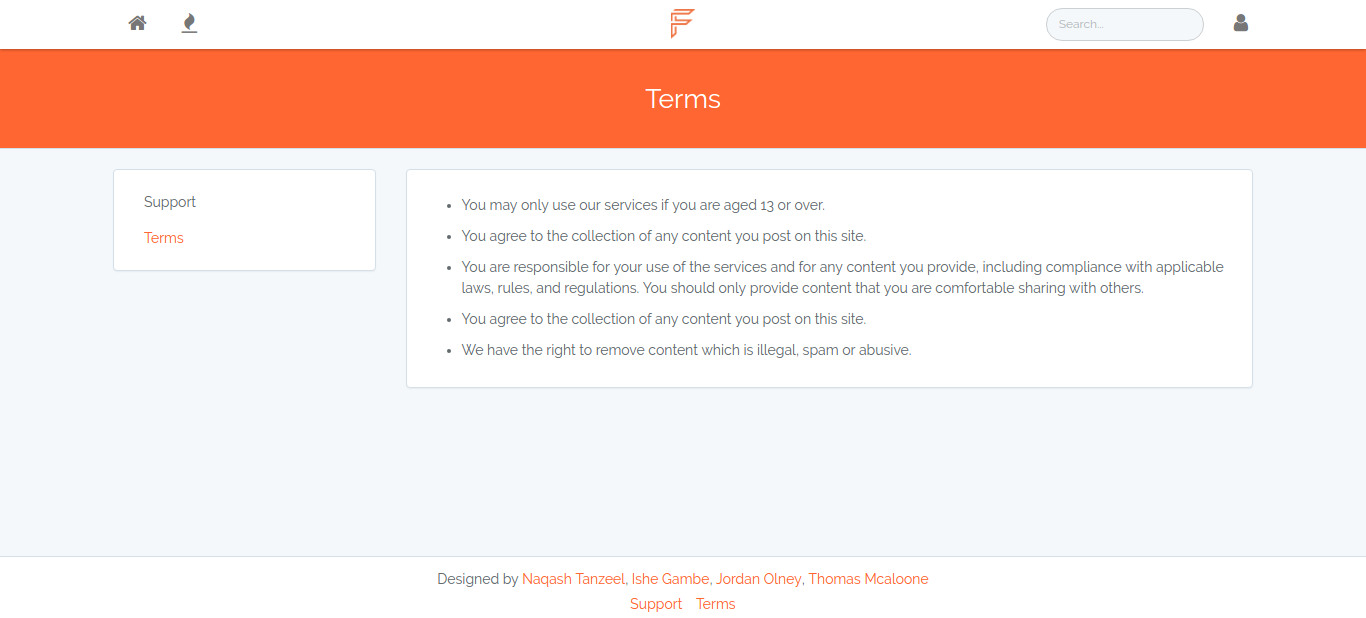
\includegraphics[height=2in]{Images/Design/terms-page}
\caption{Design for terms page}
\label{fig:ToS}
\end{figure}

\subsection{Widgets}
A public Github repository created by user \textit{arrilot} provides functionality for integrating widgets with the Laravel framework \cite{Packagist:LaravelWidgets}. The widget service provider available from this is ``a powerful alternative to view composers'', and as such using widgets is very similar to normal Laravel views. Widgets are standalone components which are composed of a class and a view. The class is responsible for all the logic and data for the widget and the view is responsible for displaying this data. To use these widgets, they must first be installed by running the following command:

\begin{lstlisting}[language=php]
 composer require arrilot/laravel-widgets
\end{lstlisting}

Once installed, the \textit{app.php} configuration must be updated with the registration of the new service provider. Widgets can be created in a similar fashion to controllers by using the Artisan utility:

\begin{lstlisting}[language=php]
 php artisan make:widget WidgetName
\end{lstlisting}

This command creates the relevant view and class for the widget. At this stage, widgets can be treated as a regular view, and can be included in existing views by using the \texttt{@widget(`widget')} directive. Parameters may optionally be passed to widgets and can be accessed in the \texttt{run()} function of the class.

\subsubsection{Profile}
The profile widget is a standalone component that display the profile information for a specified user, passed through as the second argument of the \textit{@widget()} directive. This widget is used on two separate pages, the home page, for displaying the logged in users profile, and the followers/following page, for displaying the profile of other users. These can be seen in figure \ref{fig:ProfileWidget}. The former is relatively simple as it simply uses a view to render the users details. The latter however uses slightly more complex for the following/unfollowing button. This button is rendered as a partial as it is also used on the profile page.

\begin{figure}[H]
	\centering
	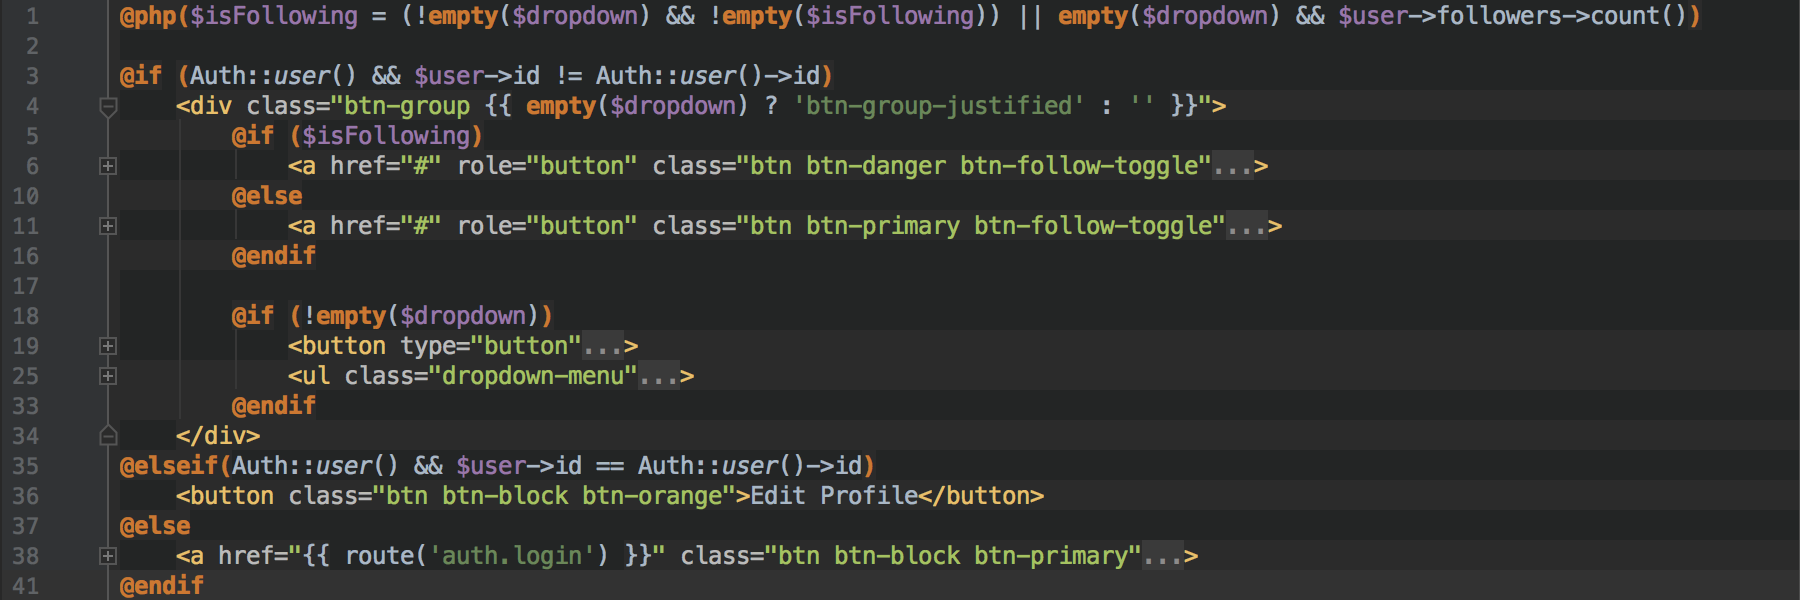
\includegraphics[width=\textwidth]{Images/Implementation/UI/Widgets/Profile_Follow}
	\caption{The code for switching the interactive button on the profile widget.}
	\label{fig:Profile_Follow}
\end{figure}

In order to display the button, we need to first determine the current relationship between the user. This is done using the logic on the first line of figure \ref{fig:Profile_Follow}. The HTML has been collapsed, which hides some of the less important code and PHP logic. Next, if we have an authorised user and this widget is not rendering the same user then we can display the follow or unfollow button based on the relationship. If the dropdown parameter has been defined as true then we add additional options such as block and unblock. If the user is viewing their own profile then we add an edit profile button but this will only occur on the profile page.

\subsubsection{Trending}
The gathering of the trending tags which is displayed by the trending widget is handled in the Trending PHP class shown in figure \ref{fig:trending-class}. The trending tags are calculated by a single database query, which selects all the tags from the post\_tags table from the last 24 hours in order of the number of posts that the tag appears within the time frame. The number of tags is then limited to 10, since this is the maximum number of tags which should be displayed in the widget. The Tag models representing these trending tags are then passed to the Blade PHP pages where the trending widget is shown so that these tags can be output to the user, allowing them to explore the tags. Because the \texttt{run()} function is called whenever a user loads a page containing the user widget, the widget will be up-to-date at the point of the user loading the page. Figure \ref{fig:trending-blade} shows the how the Blade PHP files display the tags as links to the relevant discover pages.

\begin{figure}[H]
	\centering
	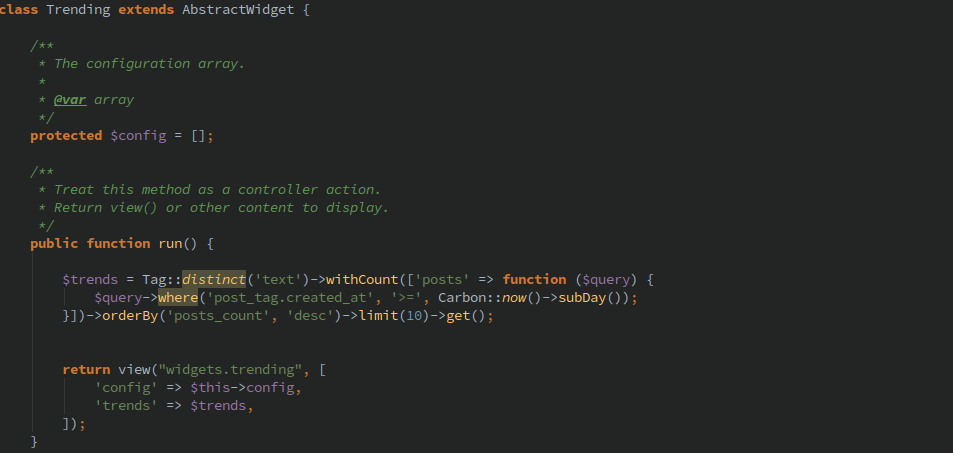
\includegraphics[width=\textwidth]{Images/Implementation/UI/Widgets/trending-class}
	\caption{The PHP class which calculates trending tags for the trending widget.}
	\label{fig:trending-class}
\end{figure}

\begin{figure}[H]
	\centering
	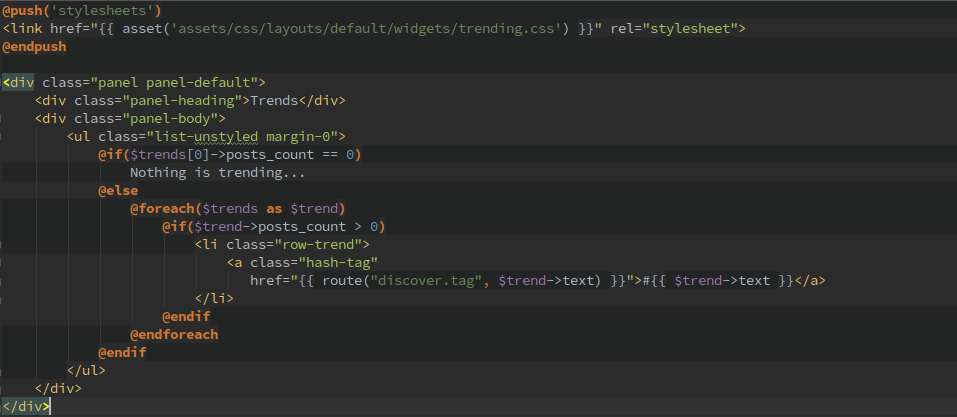
\includegraphics[width=\textwidth]{Images/Implementation/UI/Widgets/trending-blade}
	\caption{The Blade PHP file which displays the trending widget.}
	\label{fig:trending-blade}
\end{figure}

\subsubsection{Recommendations}
Figure \ref{fig:RecommendationsWidget} shows the implementation of the recommendations widget. The widget allows the user to interact with the recommendations they receive - interactions are limited to accepting or rejecting the recommendation. Additionally, users can navigate to the profile of the recommendation by clicking on their name. For both interaction types, the recommendation is removed from the widget. This ensures that the widget does not become bloated with recommendations the user has interacted with in the past, and the user is only shown recommendations they haven't responded to. Using jQuery it was possible to animate the removal of the recommendations from the widget. This provides the user with a visual cue of a successful interaction. Along with this animation, when a user accepts a recommendation the counter on the profile widget for the number of followers for the user is incremented. This again provides another visual cue to the user that their  interaction has been successful.

\begin{figure}[H]
\centering
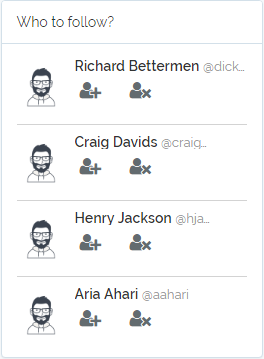
\includegraphics[height=3in]{Images/Implementation/RecommendationsWidget}
\caption{Recommendations widget}
\label{fig:RecommendationsWidget}
\end{figure}

In figure \ref{fig:UsersWidget} we can see the class for the users widget. This class is responsible for retrieving the user recommendations generated for the authorised user. Only recommendations the user has not responded to, denoted by a 0 in the database, are retrieved. 

\begin{figure}[H]
\centering
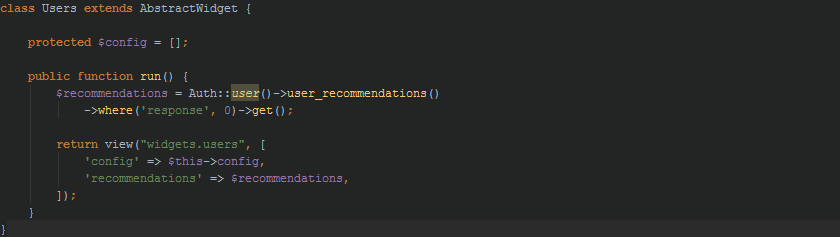
\includegraphics[width=1\textwidth]{Images/Implementation/UsersWidget}
\caption{Users widget class}
\label{fig:UsersWidget}
\end{figure}

Figure \ref{fig:UserRecommendationsController} shows the controller created for the users widget. The controller handles interactions made with recommendations. The controller extends the \textit{FollowersController}, making it possible to use the custom HTTP request \textit{FollowRequest}, which is used when a request is made to follow a user. By extending this controller, the \texttt{store()} function, which is called when the user accepts a recommendation, can log the follow request using its parents' \texttt{store()} method, and then subsequently update the response to the request. The \texttt{delete()} function is called when the user rejects one of the recommendations provided, and simply updates the response of the recommendation in the database.

\begin{figure}[H]
\centering
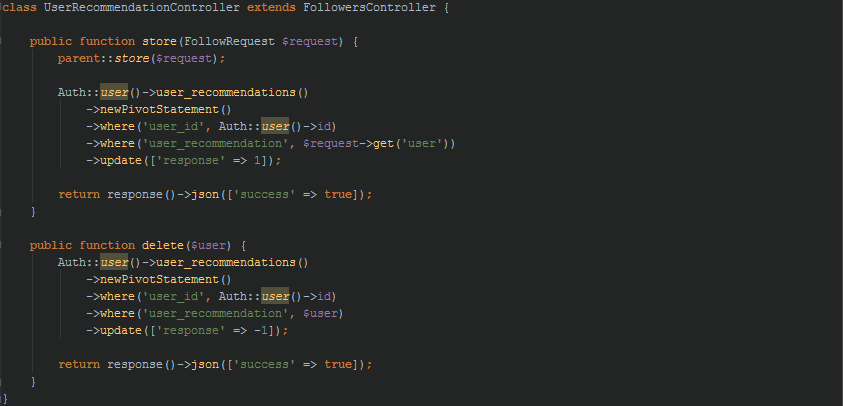
\includegraphics[width=1\textwidth]{Images/Implementation/UserRecommendationsController}
\caption{Users widget class}
\label{fig:UserRecommendationsController}
\end{figure}